\documentclass[11pt]{article}

\usepackage[a4paper]{geometry}
\geometry{left=2.0cm,right=2.0cm,top=3cm,bottom=2.5cm}
\usepackage{setspace}
\setstretch{1.5}
\usepackage{ctex}
\usepackage{amsmath,amsfonts,graphicx,amssymb,bm,amsthm}
\usepackage{algorithm,algorithmicx}
\usepackage[noend]{algpseudocode}
\usepackage{fancyhdr}
\usepackage{booktabs}
\usepackage{array}
\usepackage{listings}
\usepackage{listingsutf8}
\usepackage{xcolor}
\lstset{
	language=Python,
	basicstyle=\ttfamily\small,
	numbers=left,
	numberstyle=\tiny\color{teal!70!black},
	showstringspaces=false,
	breaklines=true,
	frame=single,
	rulecolor=\color{black},
	framerule=0.6pt,
	framesep=4pt,
	xleftmargin=6pt,
	backgroundcolor=\color{gray!4},
	inputencoding=utf8,
	columns=fullflexible,
	keywordstyle=\bfseries\color{blue!70!black},
	commentstyle=\itshape\color{green!50!black},
	stringstyle=\color{red!60!black},
	identifierstyle=\color{violet!70!black},
	emphstyle=\bfseries\color{orange!80!black},
	tabsize=4
}
\newcolumntype{M}[1]{>{\centering\arraybackslash}m{#1}}
\begin{document}
	\pagestyle{fancy}
	\lhead{\kaishu 中国科学院大学}
	\chead{}
	\rhead{\kaishu 2025年秋季学期\qquad 人工智能原理：模型与算法}
	
	\begin{center}
		{\LARGE \bf 课程作业3} 
	\end{center}
	\begin{center}
		\large\kaishu{尧祥临 202518023406038 前沿交叉科学学院}
	\end{center}

	\section{任务介绍}
	本次作业旨在构建一个基于私有知识库的问答系统（RAG），主要的要求分为三层：
	\begin{enumerate}
		\item 应用构建平台 Dify，快速部署对话问答系统。
		\item 通过Ollama在本地部署推理大模型和嵌入模型实现数据的隐私保护和本地化运行。
		\item 在完成基础RAG系统后，尝试基于知识图谱的检索增强生成。
	\end{enumerate}

	由于在第三层的知识图谱构建中遇到了一些环境配置的问题，导致未能成功实现该部分内容，未来会继续探索实现，但是在这一次作业中暂时只完成前两层的任务。

	\section{环境配置与模型选择}
	\subsection{Dify环境搭建}
	按照ppt要求，我在Windows 10系统的WSL2子系统中，首先配置了Docker环境，具体而言包括安装 Docker Desktop for Windows，并启用WSL2后端支持。然后在WSL2中安装DockerCLI和Docker Compose插件。之后，在docker中拉取并运行Dify的Docker镜像，实现Dify平台的本地部署。完成后，通过浏览器访问 \texttt{http://localhost/install}，成功进入Dify平台首页。

	\subsection{本地模型部署 (Ollama)}
	课件中建议第一层使用deepseek的API，但考虑到本地硬件资源允许，这里选择跳过第一层基于API的问答系统，而是直接利用Ollama在本地部署大语言模型以及嵌入模型。其中大语言模型采用推荐的deepseek-r1:7b，嵌入模型同样采用了推荐的nomic-embed-text:v1.5，该模型用于将知识库文本转化为向量，是实现RAG检索的关键。

	\begin{figure}[htbp]
	     \centering
	     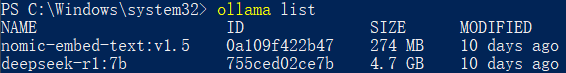
\includegraphics[width=0.8\textwidth]{../Figure/Ollama.png} % 替换为你的截图文件名
	     \caption{Ollama本地模型列表}
	\end{figure}

	\subsection{Dify 与 Ollama 的连接}
	为了让运行在 Docker 容器内的 Dify 能够访问宿主机的 Ollama 服务，这里需要在 Dify 的模型供应商设置中，将Base URL配置为 \texttt{http://host.docker.internal:11434}。配置完成后，成功添加了 LLM和Text Embedding模型。

    \begin{figure}[htbp]
         \centering
         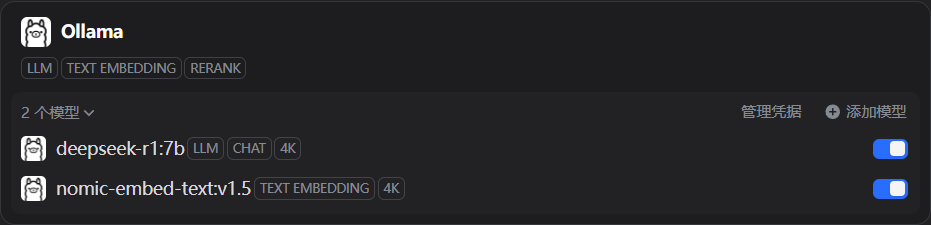
\includegraphics[width=0.8\textwidth]{../Figure/Models.png} % 替换为你的截图文件名
         \caption{Dify模型配置}
    \end{figure}

	\section{知识库构建与对话效果展示}
	
	\subsection{知识库构建}
	在 Dify 的知识库界面中中创建了名为“复杂网络的统计描述”新知识库，并上传了相关的PDF格式的文献文档作为知识库的原始数据。其中在上传文件的时候，选择了通用的分段模式，同时设置为高质量索引模式，调用本地部署好的 嵌入模型来处理文档，并设置为向量检索，Top K为3，Score为阈值为0.5。

    \begin{figure}[htbp]
         \centering
         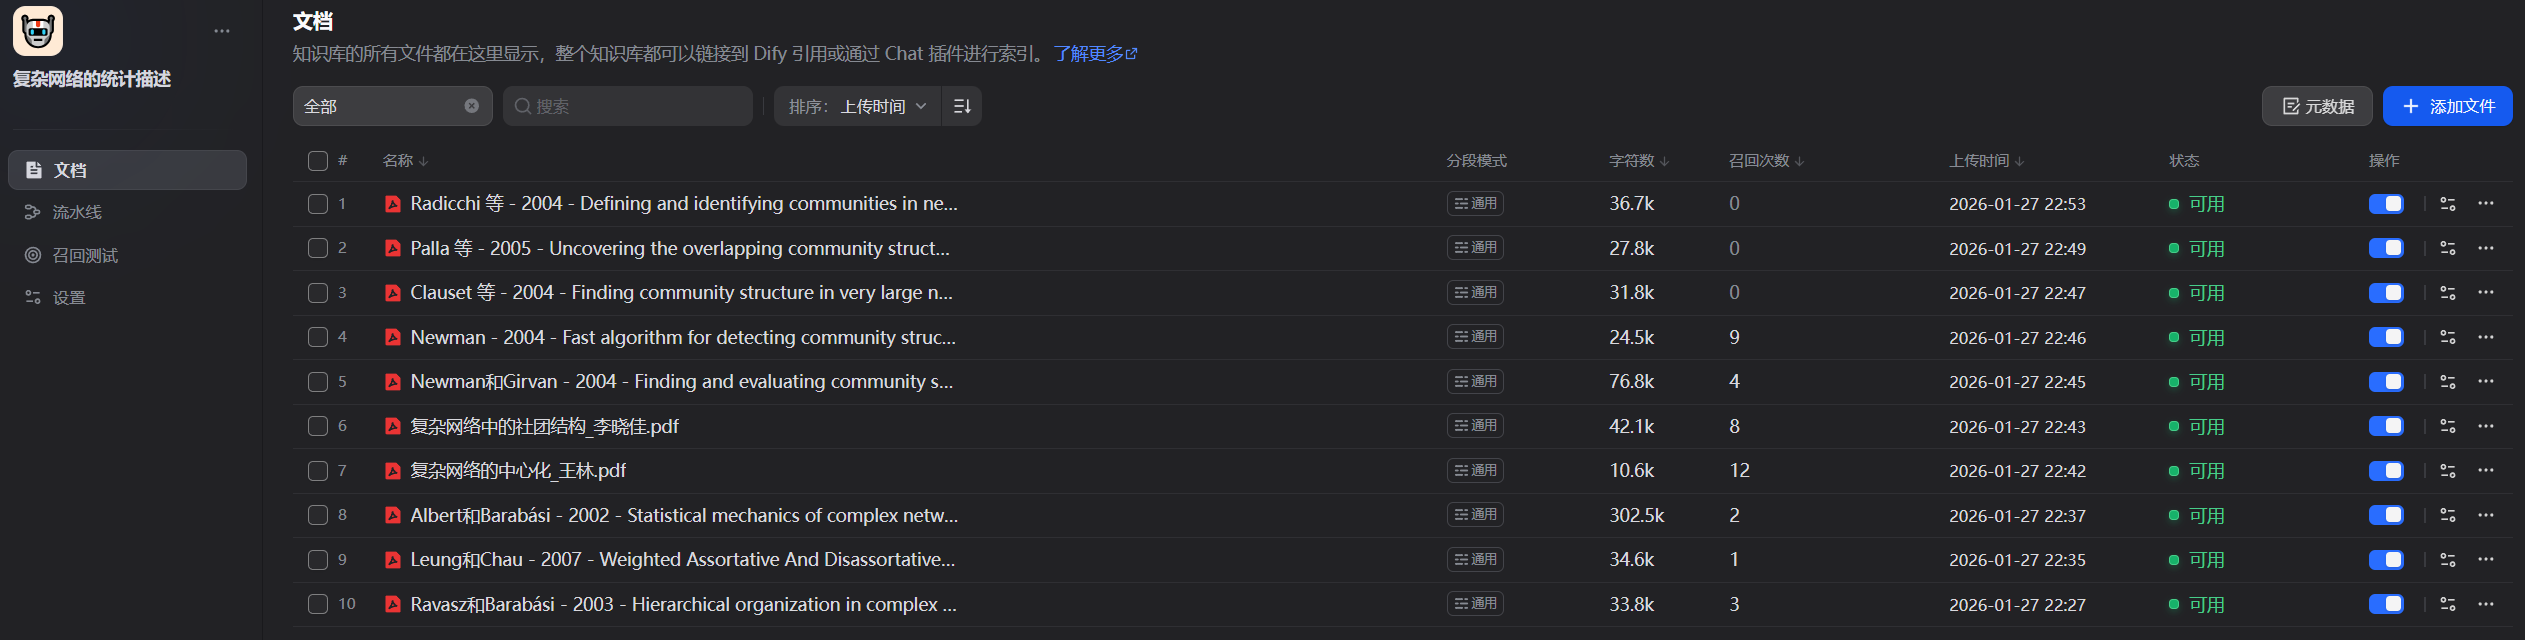
\includegraphics[width=0.8\textwidth]{../Figure/Files.png}
         \caption{知识库构建}
    \end{figure}

	\subsection{应用编排与对话测试}
	在Dify的工作室中创建了一个“知识问答系统v1.0”的应用，使用本地部署的deepseek模型，并关联了上述构建的知识库。配置完成后开始进行对话测试，经过几个问题的尝试，我发现了当前问答系统存在的一些现象和问题。

	如图\ref{fig:Talk1}所示，当我询问模型“介数中心性是什么？”的时候，模型除了能从知识库中检索到相应的定义和描述，很大一部分的输出内容应该是来自于模型本身的知识储备，说明模型在回答问题时会综合利用检索到的内容和自身的预训练知识。图\ref{fig:Search1}所示的为模型对于这个问题提供的参考的文献片段，可以看到模型成功地从知识库中检索到了相关内容，并将其作为回答的一部分。

    \begin{figure}[htbp]
         \centering
         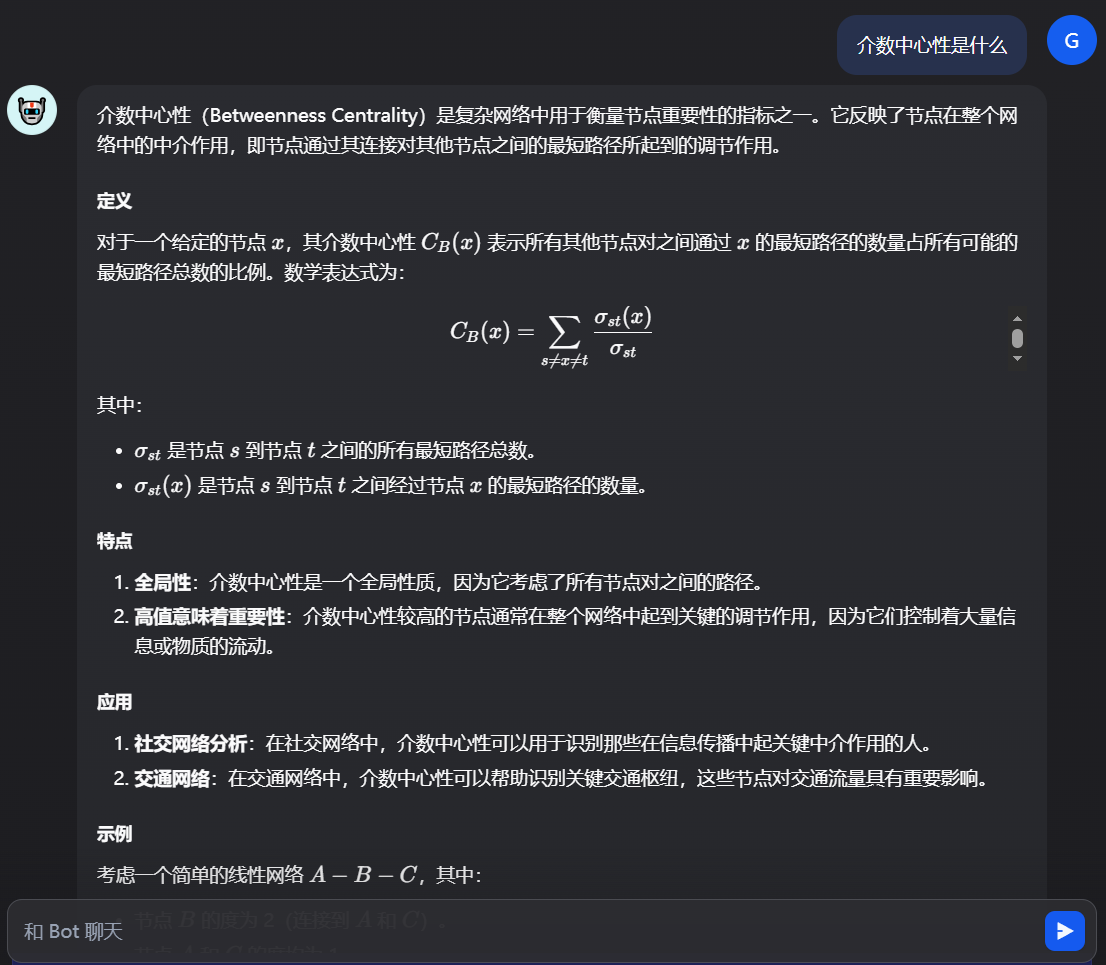
\includegraphics[width=0.7\textwidth]{../Figure/Talk1.png}
         \caption{第一个问题}
		 \label{fig:Talk1}
    \end{figure}

	\begin{figure}[htbp]
         \centering
         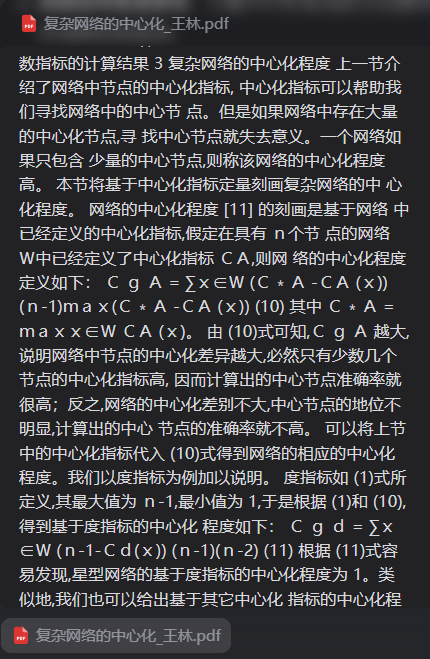
\includegraphics[width=0.4\textwidth]{../Figure/Search1.png}
         \caption{第一个问题的文献片段检索结果}
		 \label{fig:Search1}
    \end{figure}

	但是并不是所有问题都能够正确检索到结果，如图\ref{fig:Talk2}所示，当询问模型“复杂网络的效率是什么？”的时候，模型虽然根据其预训练知识给出了一个合理的定义，但并没有从知识库中检索到内容实际上都并不相关。例如图\ref{fig:Search2}所示的三个结果，模型实际上检索的关键词是“复杂网络”，而并非是问题中更关键的“效率”。事实上，这个问题在知识库中来自一篇英文文献，图所示的为在英文文献中该概念对应的位置，说明当前的知识库构建和检索机制在处理多语言文档时还存在一定的不足，这更多可能与两个本地部署的模型对于多语言的支持能力不够强有关。
	\begin{figure}[htbp]
         \centering
         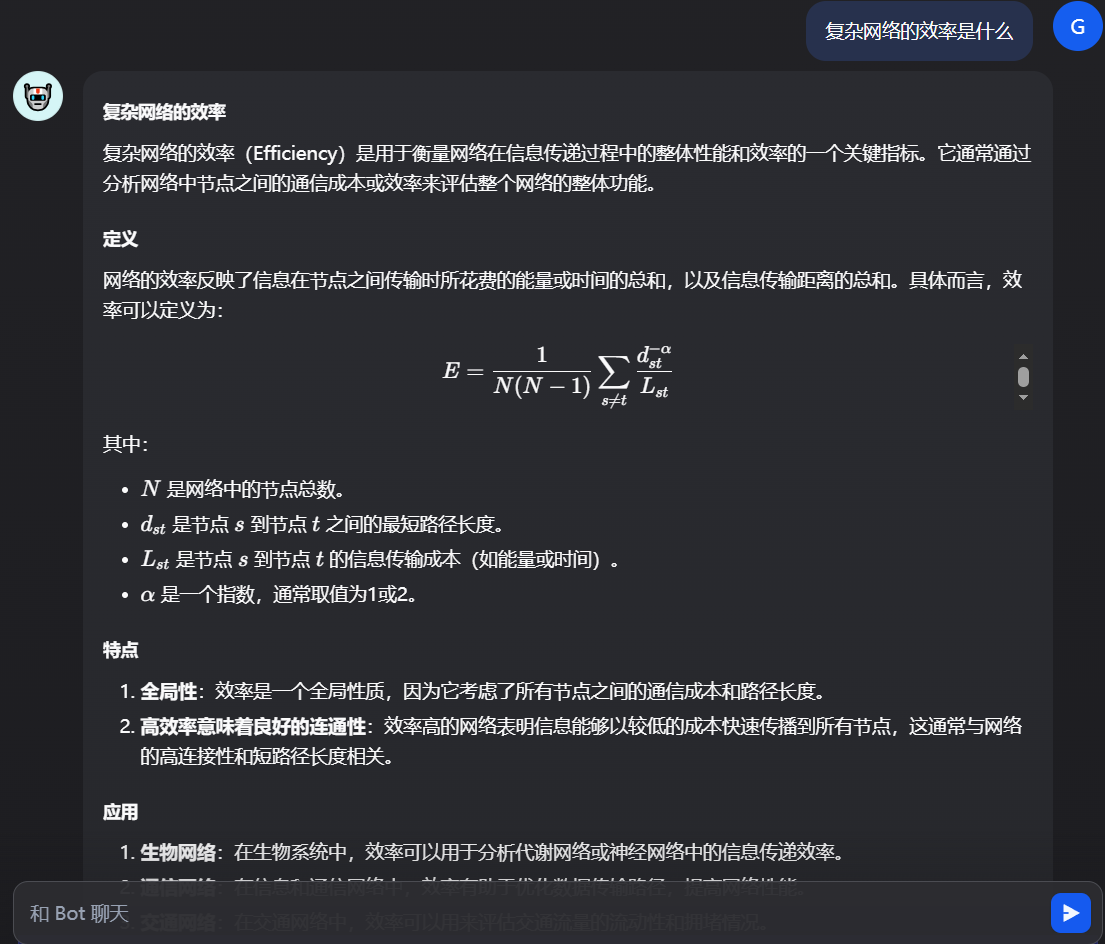
\includegraphics[width=0.7\textwidth]{../Figure/Talk2.png}
         \caption{第二个问题}
		 \label{fig:Talk2}
    \end{figure}

	\begin{figure}[htbp]
		\centering
		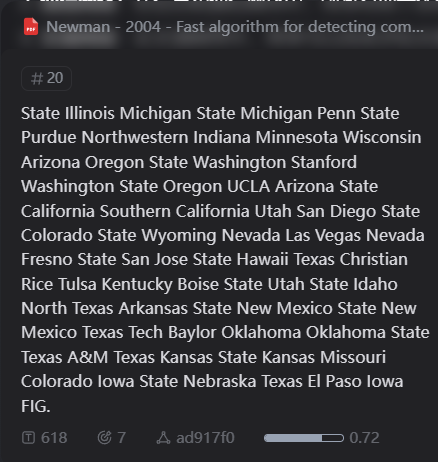
\includegraphics[width=0.32\textwidth]{../Figure/Search2-1.png}
		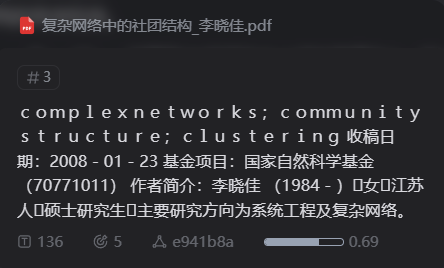
\includegraphics[width=0.32\textwidth]{../Figure/Search2-2.png}
		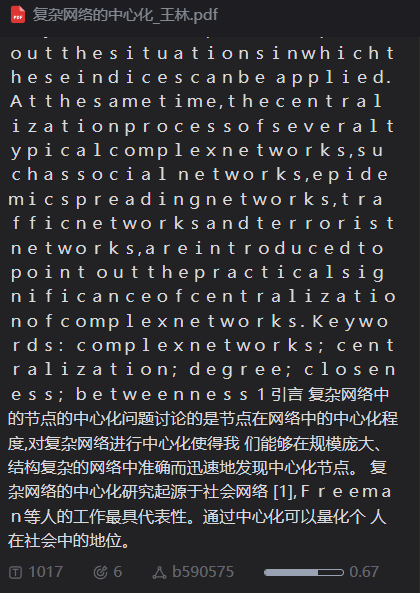
\includegraphics[width=0.32\textwidth]{../Figure/Search2-3.png}
		\caption{第二个问题的文献片段检索结果}
		\label{fig:Search2}
	\end{figure}

	\begin{figure}[htbp]
         \centering
         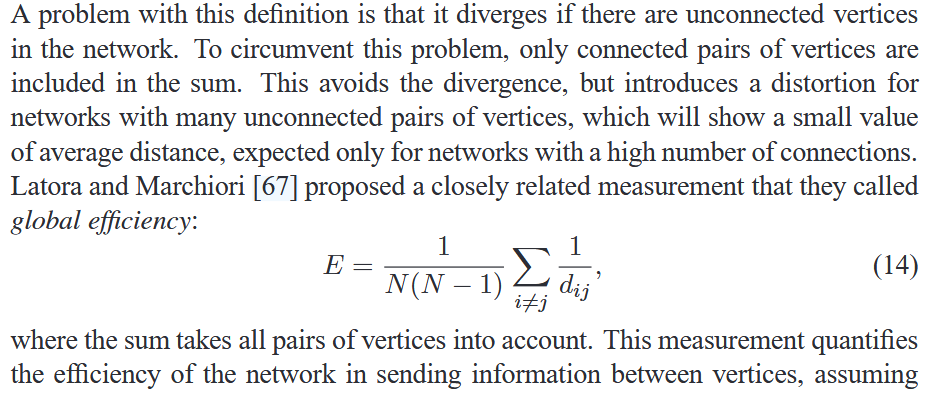
\includegraphics[width=0.7\textwidth]{../Figure/Talk2file.png}
         \caption{复杂网络的效率的定义在英文文献中的位置}
		 \label{fig:Talk2file}
    \end{figure}

    \section{总结}
    
    本次作业成功搭建了一套完全基于本地环境的RAG知识问答系统。实现了 Dify平台与Ollama本地模型的集成；在完成基础RAG构建后，我尝试进一步探索基于知识图谱的检索增强生成。在WSL2环境中配置Python服务端并尝试构建图谱索引时，遇到一些版本兼容性问题，导致服务无法稳定运行。鉴于基础RAG系统已满足作业核心需求，因此本次报告主要展示基于向量检索的成果，之后若有机会会继续完善知识图谱部分。
\end{document}